\documentclass[si.tex]{subfiles}
\begin{document}

\paragraph*{Theoretical Discussion}
While our Theorems 3 and 4 apply in the setting where the encoding is shared between noise levels, here we discuss the case where the encoding varies between noise levels.
For each noise level $\sigma$ and associated encoding $F'_\sigma$, we have the model $M_\sigma := \langle F'_\sigma, \Prior, p\rangle$, where $p$ is the loss function exponent.
We first discuss the case without motor noise. Here, Theorem 1 can be used to recover the encoding in each noise level to high accuracy.
Theorem 2 can then be used to obtain the prior, conditional on the loss function exponent.
By comparing the bias at each noise level $\sigma$ to the expansion from Lemma~\ref{lemma:expansion}, we can expect to recover the loss function exponent $p$ for most models outside of a small exceptional set, similar to the set $\Omega$ of Theorem 3.
The situation is more complex in the presence of motor noise. A general approach is to deconvolve the response distribution with a motor variance $\tau^2$, and then apply the same reasoning as above. While $\tau^2$ is unknown, one may expect that only one possible $\tau^2$ may lead to a consistent result, at least on models outside of a small exceptional set. Thus, we expect that the theoretical guarantees of Theorems 3 and 4 extend to many models where the encoding varies between noise levels.


\paragraph*{Simulations}
Here, we evaluate the identifiability of models on the situation where the shape of the encoding may itself depend on the noise level.
We considered a situation where the encodings are similar across noise levels, but vary in their steepness (Figure~\ref{fig:encoding-varies-additive}), and where they are independent (Figure~\ref{fig:encoding-varies-fourier}).



\begin{comment}

# Creating datasets and fits (already done)
#python3 SimulateSynthetic_Parameterized_OtherNoiseLevels_Grid_VarySize_SeparateEncodings.py 2 0 10.0 180 40000 UNIFORM FOURIER_210-FOURIER_211-FOURIER_212-FOURIER_213 2345
#python3 SimulateSynthetic_Parameterized_OtherNoiseLevels_Grid_VarySize_SeparateEncodings.py 4 0 10.0 180 40000 UNIFORM FOURIER_410-FOURIER_411-FOURIER_412-FOURIER_413 2345
#python3 SimulateSynthetic_Parameterized_OtherNoiseLevels_Grid_VarySize_SeparateEncodings.py 6 0 10.0 180 40000 UNIFORM FOURIER_610-FOURIER_611-FOURIER_612-FOURIER_613 2345
#python3 SimulateSynthetic_Parameterized_OtherNoiseLevels_Grid_VarySize_SeparateEncodings.py 8 0 10.0 180 40000 UNIFORM FOURIER_810-FOURIER_811-FOURIER_812-FOURIER_813 2345
#
#python3 SimulateSynthetic_Parameterized_OtherNoiseLevels_Grid_VarySize_SeparateEncodings.py 2 0 10.0 180 40000 FOURIER_209 FOURIER_210-FOURIER_211-FOURIER_212-FOURIER_213 2345
#python3 SimulateSynthetic_Parameterized_OtherNoiseLevels_Grid_VarySize_SeparateEncodings.py 4 0 10.0 180 40000 FOURIER_409 FOURIER_410-FOURIER_411-FOURIER_412-FOURIER_413 2345
#python3 SimulateSynthetic_Parameterized_OtherNoiseLevels_Grid_VarySize_SeparateEncodings.py 6 0 10.0 180 40000 FOURIER_609 FOURIER_610-FOURIER_611-FOURIER_612-FOURIER_613 2345
#python3 SimulateSynthetic_Parameterized_OtherNoiseLevels_Grid_VarySize_SeparateEncodings.py 8 0 10.0 180 40000 FOURIER_809 FOURIER_810-FOURIER_811-FOURIER_812-FOURIER_813 2345
#
#



# Creating plots

python3 RunSynthetic_FreePrior_ZeroTrig_OnSim_SeparateEncoding_VIZ.py 0 0 10.0 180 SimulateSynthetic_Parameterized_OtherNoiseLevels_Grid_VarySize_ZeroTrig_AdditiveEncodings.py_180_0_2345_N40000_STEEPPERIODIC_STEEPPERIODIC.txt
python3 RunSynthetic_FreePrior_L1Loss_OnSim_SeparateEncoding_VIZ.py 1 0 10.0 180 SimulateSynthetic_Parameterized_OtherNoiseLevels_Grid_VarySize_AdditiveEncodings.py_180_1_2345_N40000_STEEPPERIODIC_STEEPPERIODIC.txt
python3 RunSynthetic_FreePrior_CosineLoss_OnSim_SeparateEncoding_VIZ.py 2 0 10.0 180 SimulateSynthetic_Parameterized_OtherNoiseLevels_Grid_VarySize_AdditiveEncodings.py_180_2_2345_N40000_STEEPPERIODIC_STEEPPERIODIC.txt
python3 RunSynthetic_FreePrior_CosineLoss_OnSim_SeparateEncoding_VIZ.py 4 0 10.0 180 SimulateSynthetic_Parameterized_OtherNoiseLevels_Grid_VarySize_AdditiveEncodings.py_180_4_2345_N40000_STEEPPERIODIC_STEEPPERIODIC.txt
python3 RunSynthetic_FreePrior_CosineLoss_OnSim_SeparateEncoding_VIZ.py 6 0 10.0 180 SimulateSynthetic_Parameterized_OtherNoiseLevels_Grid_VarySize_AdditiveEncodings.py_180_6_2345_N40000_STEEPPERIODIC_STEEPPERIODIC.txt
python3 RunSynthetic_FreePrior_CosineLoss_OnSim_SeparateEncoding_VIZ.py 8 0 10.0 180 SimulateSynthetic_Parameterized_OtherNoiseLevels_Grid_VarySize_AdditiveEncodings.py_180_8_2345_N40000_STEEPPERIODIC_STEEPPERIODIC.txt

python3 CounterfactualModel_AdditiveEncodings_VIZ.py 0 0 10.0 180 STEEPPERIODIC STEEPPERIODIC 2345
python3 CounterfactualModel_AdditiveEncodings_VIZ.py 1 0 10.0 180 STEEPPERIODIC STEEPPERIODIC 2345
python3 CounterfactualModel_AdditiveEncodings_VIZ.py 2 0 10.0 180 STEEPPERIODIC STEEPPERIODIC 2345
python3 CounterfactualModel_AdditiveEncodings_VIZ.py 4 0 10.0 180 STEEPPERIODIC STEEPPERIODIC 2345
python3 CounterfactualModel_AdditiveEncodings_VIZ.py 6 0 10.0 180 STEEPPERIODIC STEEPPERIODIC 2345
python3 CounterfactualModel_AdditiveEncodings_VIZ.py 8 0 10.0 180 STEEPPERIODIC STEEPPERIODIC 2345





#python3 RunSynthetic_FreePrior_CosineLoss_OnSim_SeparateEncoding_VIZ.py 2 0 10.0 180 SimulateSynthetic_Parameterized_OtherNoiseLevels_Grid_VarySize_AdditiveEncodings.py_180_2_2345_N40000_UNIFORM_STEEPPERIODIC.txt
#python3 RunSynthetic_FreePrior_CosineLoss_OnSim_SeparateEncoding_VIZ.py 4 0 10.0 180 SimulateSynthetic_Parameterized_OtherNoiseLevels_Grid_VarySize_AdditiveEncodings.py_180_4_2345_N40000_UNIFORM_STEEPPERIODIC.txt
#python3 RunSynthetic_FreePrior_CosineLoss_OnSim_SeparateEncoding_VIZ.py 6 0 10.0 180 SimulateSynthetic_Parameterized_OtherNoiseLevels_Grid_VarySize_AdditiveEncodings.py_180_6_2345_N40000_UNIFORM_STEEPPERIODIC.txt
#python3 RunSynthetic_FreePrior_CosineLoss_OnSim_SeparateEncoding_VIZ.py 8 0 10.0 180 SimulateSynthetic_Parameterized_OtherNoiseLevels_Grid_VarySize_AdditiveEncodings.py_180_8_2345_N40000_UNIFORM_STEEPPERIODIC.txt

\end{comment}

\begin{comment}
#python3 SimulateSynthetic_Parameterized_OtherNoiseLevels_Grid_VarySize_ZeroTrig_AdditiveEncodings.py 0 0 10.0 180 40000 STEEPPERIODIC STEEPPERIODIC 2345
#python3 SimulateSynthetic_Parameterized_OtherNoiseLevels_Grid_VarySize_ZeroTrig_AdditiveEncodings.py 0 0 10.0 180 40000 UNIFORM STEEPPERIODIC 2345
#python3 SimulateSynthetic_Parameterized_OtherNoiseLevels_Grid_VarySize_AdditiveEncodings.py 1 0 10.0 180 40000 STEEPPERIODIC STEEPPERIODIC 2345
#python3 SimulateSynthetic_Parameterized_OtherNoiseLevels_Grid_VarySize_AdditiveEncodings.py 1 0 10.0 180 40000 UNIFORM STEEPPERIODIC 2345
#
#
#python3 SimulateSynthetic_Parameterized_OtherNoiseLevels_Grid_VarySize_SeparateEncodings.py 1 0 10.0 180 40000 FOURIER_109 FOURIER_110-FOURIER_111-FOURIER_112-FOURIER_113 2345
#python3 SimulateSynthetic_Parameterized_OtherNoiseLevels_Grid_VarySize_SeparateEncodings.py 1 0 10.0 180 40000 UNIFORM FOURIER_110-FOURIER_111-FOURIER_112-FOURIER_113 2345
#python3 SimulateSynthetic_Parameterized_OtherNoiseLevels_Grid_VarySize_ZeroTrig_SeparateEncodings.py 0 0 10.0 180 40000 FOURIER_009 FOURIER_010-FOURIER_011-FOURIER_012-FOURIER_013 2345
#python3 SimulateSynthetic_Parameterized_OtherNoiseLevels_Grid_VarySize_ZeroTrig_SeparateEncodings.py 0 0 10.0 180 40000 UNIFORM FOURIER_010-FOURIER_011-FOURIER_012-FOURIER_013 2345


python3 RunSynthetic_FreePrior_CosineLoss_OnSim_SeparateEncoding_VIZ.py 2 0 10.0 180 SimulateSynthetic_Parameterized_OtherNoiseLevels_Grid_VarySize_SeparateEncodings.py_180_2_2345_N40000_FOURIER_209_FOURIER_210-FOURIER_211-FOURIER_212-FOURIER_213.txt
python3 RunSynthetic_FreePrior_CosineLoss_OnSim_SeparateEncoding_VIZ.py 2 0 10.0 180 SimulateSynthetic_Parameterized_OtherNoiseLevels_Grid_VarySize_SeparateEncodings.py_180_2_2345_N40000_UNIFORM_FOURIER_210-FOURIER_211-FOURIER_212-FOURIER_213.txt
python3 RunSynthetic_FreePrior_CosineLoss_OnSim_SeparateEncoding_VIZ.py 4 0 10.0 180 SimulateSynthetic_Parameterized_OtherNoiseLevels_Grid_VarySize_SeparateEncodings.py_180_4_2345_N40000_FOURIER_409_FOURIER_410-FOURIER_411-FOURIER_412-FOURIER_413.txt
python3 RunSynthetic_FreePrior_CosineLoss_OnSim_SeparateEncoding_VIZ.py 4 0 10.0 180 SimulateSynthetic_Parameterized_OtherNoiseLevels_Grid_VarySize_SeparateEncodings.py_180_4_2345_N40000_UNIFORM_FOURIER_410-FOURIER_411-FOURIER_412-FOURIER_413.txt
python3 RunSynthetic_FreePrior_CosineLoss_OnSim_SeparateEncoding_VIZ.py 6 0 10.0 180 SimulateSynthetic_Parameterized_OtherNoiseLevels_Grid_VarySize_SeparateEncodings.py_180_6_2345_N40000_FOURIER_609_FOURIER_610-FOURIER_611-FOURIER_612-FOURIER_613.txt
python3 RunSynthetic_FreePrior_CosineLoss_OnSim_SeparateEncoding_VIZ.py 6 0 10.0 180 SimulateSynthetic_Parameterized_OtherNoiseLevels_Grid_VarySize_SeparateEncodings.py_180_6_2345_N40000_UNIFORM_FOURIER_610-FOURIER_611-FOURIER_612-FOURIER_613.txt
python3 RunSynthetic_FreePrior_CosineLoss_OnSim_SeparateEncoding_VIZ.py 8 0 10.0 180 SimulateSynthetic_Parameterized_OtherNoiseLevels_Grid_VarySize_SeparateEncodings.py_180_8_2345_N40000_FOURIER_809_FOURIER_810-FOURIER_811-FOURIER_812-FOURIER_813.txt
python3 RunSynthetic_FreePrior_CosineLoss_OnSim_SeparateEncoding_VIZ.py 8 0 10.0 180 SimulateSynthetic_Parameterized_OtherNoiseLevels_Grid_VarySize_SeparateEncodings.py_180_8_2345_N40000_UNIFORM_FOURIER_810-FOURIER_811-FOURIER_812-FOURIER_813.txt

\end{comment}



\begin{comment}
#runForFigure5_SeparateEncoding.py
#runForFigure5_SeparateEncoding_Zero.py
#runForFigure5_SeparateEncoding_L1.py

python3 RunSynthetic_FreePrior_CosineLoss_OnSim_SeparateEncoding_VIZ.py 2 0 10.0 180 SimulateSynthetic_Parameterized_OtherNoiseLevels_Grid_VarySize_AdditiveEncodings.py_180_2_2345_N40000_STEEPPERIODIC_STEEPPERIODIC.txt
python3 RunSynthetic_FreePrior_CosineLoss_OnSim_SeparateEncoding_VIZ.py 4 0 10.0 180 SimulateSynthetic_Parameterized_OtherNoiseLevels_Grid_VarySize_AdditiveEncodings.py_180_4_2345_N40000_STEEPPERIODIC_STEEPPERIODIC.txt
python3 RunSynthetic_FreePrior_CosineLoss_OnSim_SeparateEncoding_VIZ.py 6 0 10.0 180 SimulateSynthetic_Parameterized_OtherNoiseLevels_Grid_VarySize_AdditiveEncodings.py_180_6_2345_N40000_STEEPPERIODIC_STEEPPERIODIC.txt
python3 RunSynthetic_FreePrior_CosineLoss_OnSim_SeparateEncoding_VIZ.py 8 0 10.0 180 SimulateSynthetic_Parameterized_OtherNoiseLevels_Grid_VarySize_AdditiveEncodings.py_180_8_2345_N40000_STEEPPERIODIC_STEEPPERIODIC.txt

\end{comment}

\begin{figure}
    \centering


  \begin{minipage}[b]{0.45\linewidth}
    \centering



$p=0$

\sideimage{Original}{figures/CounterfactualModel_AdditiveEncodings_VIZ.py_2345_STEEPPERIODIC_STEEPPERIODIC_0_0_10.0_180.pdf}	

\sideimage{Fitted}{figures/RunSynthetic_FreePrior_ZeroTrig_OnSim_SeparateEncoding_VIZ.py_SimulateSynthetic_Parameterized_OtherNoiseLevels_Grid_VarySize_ZeroTrig_AdditiveEncodings.py_180_0_2345_N40000_STEEPPERIODIC_STEEPPERIODIC.txt_0_0_10.0_180.pdf}

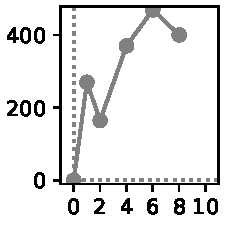
\includegraphics[width=0.3\textwidth]{figures/evaluateCrossValidationResults_Synthetic_Gardelle_NonF_SeparateEncoding.py_SimulateSynthetic_Parameterized_OtherNoiseLevels_Grid_VarySize_ZeroTrig_AdditiveEncodings.py_180_0_2345_N40000_STEEPPERIODIC_STEEPPERIODIC.txt_RelativeLF.pdf}


\ 

$p=1$

\sideimage{Original}{figures/CounterfactualModel_AdditiveEncodings_VIZ.py_2345_STEEPPERIODIC_STEEPPERIODIC_1_0_10.0_180.pdf}	



\sideimage{Fitted}{figures/RunSynthetic_FreePrior_L1Loss_OnSim_SeparateEncoding_VIZ.py_SimulateSynthetic_Parameterized_OtherNoiseLevels_Grid_VarySize_AdditiveEncodings.py_180_1_2345_N40000_STEEPPERIODIC_STEEPPERIODIC.txt_1_0_10.0_180.pdf}


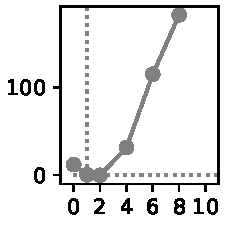
\includegraphics[width=0.3\textwidth]{figures/evaluateCrossValidationResults_Synthetic_Gardelle_NonF_SeparateEncoding.py_SimulateSynthetic_Parameterized_OtherNoiseLevels_Grid_VarySize_AdditiveEncodings.py_180_1_2345_N40000_STEEPPERIODIC_STEEPPERIODIC.txt_RelativeLF.pdf}

\ 

$p=2$

\sideimage{Original}{figures/CounterfactualModel_AdditiveEncodings_VIZ.py_2345_STEEPPERIODIC_STEEPPERIODIC_2_0_10.0_180.pdf}	
\sideimage{Fitted}{figures/RunSynthetic_FreePrior_CosineLoss_OnSim_SeparateEncoding_VIZ.py_SimulateSynthetic_Parameterized_OtherNoiseLevels_Grid_VarySize_AdditiveEncodings.py_180_2_2345_N40000_STEEPPERIODIC_STEEPPERIODIC.txt_2_0_10.0_180.pdf}
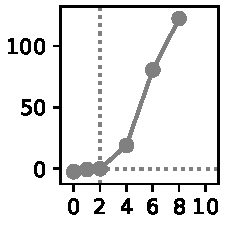
\includegraphics[width=0.3\textwidth]{figures/evaluateCrossValidationResults_Synthetic_Gardelle_NonF_SeparateEncoding.py_SimulateSynthetic_Parameterized_OtherNoiseLevels_Grid_VarySize_AdditiveEncodings.py_180_2_2345_N40000_STEEPPERIODIC_STEEPPERIODIC.txt_RelativeLF.pdf}

  \end{minipage}%
  \hfill
  \begin{minipage}[b]{0.45\linewidth}
    \centering

$p=4$

\sideimage{Original}{figures/CounterfactualModel_AdditiveEncodings_VIZ.py_2345_STEEPPERIODIC_STEEPPERIODIC_4_0_10.0_180.pdf}	
\sideimage{Fitted}{figures/RunSynthetic_FreePrior_CosineLoss_OnSim_SeparateEncoding_VIZ.py_SimulateSynthetic_Parameterized_OtherNoiseLevels_Grid_VarySize_AdditiveEncodings.py_180_4_2345_N40000_STEEPPERIODIC_STEEPPERIODIC.txt_4_0_10.0_180.pdf}

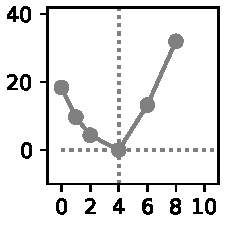
\includegraphics[width=0.3\textwidth]{figures/evaluateCrossValidationResults_Synthetic_Gardelle_NonF_SeparateEncoding.py_SimulateSynthetic_Parameterized_OtherNoiseLevels_Grid_VarySize_AdditiveEncodings.py_180_4_2345_N40000_STEEPPERIODIC_STEEPPERIODIC.txt_RelativeLF.pdf}

\ 

$p=6$

\sideimage{Original}{figures/CounterfactualModel_AdditiveEncodings_VIZ.py_2345_STEEPPERIODIC_STEEPPERIODIC_6_0_10.0_180.pdf}	
\sideimage{Fitted}{figures/RunSynthetic_FreePrior_CosineLoss_OnSim_SeparateEncoding_VIZ.py_SimulateSynthetic_Parameterized_OtherNoiseLevels_Grid_VarySize_AdditiveEncodings.py_180_6_2345_N40000_STEEPPERIODIC_STEEPPERIODIC.txt_6_0_10.0_180.pdf}
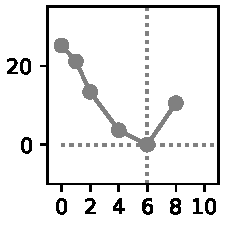
\includegraphics[width=0.3\textwidth]{figures/evaluateCrossValidationResults_Synthetic_Gardelle_NonF_SeparateEncoding.py_SimulateSynthetic_Parameterized_OtherNoiseLevels_Grid_VarySize_AdditiveEncodings.py_180_6_2345_N40000_STEEPPERIODIC_STEEPPERIODIC.txt_RelativeLF.pdf}

\ 

$p=8$

\sideimage{Original}{figures/CounterfactualModel_AdditiveEncodings_VIZ.py_2345_STEEPPERIODIC_STEEPPERIODIC_8_0_10.0_180.pdf}	
\sideimage{Fitted}{figures/RunSynthetic_FreePrior_CosineLoss_OnSim_SeparateEncoding_VIZ.py_SimulateSynthetic_Parameterized_OtherNoiseLevels_Grid_VarySize_AdditiveEncodings.py_180_8_2345_N40000_STEEPPERIODIC_STEEPPERIODIC.txt_8_0_10.0_180.pdf}
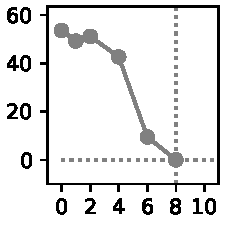
\includegraphics[width=0.3\textwidth]{figures/evaluateCrossValidationResults_Synthetic_Gardelle_NonF_SeparateEncoding.py_SimulateSynthetic_Parameterized_OtherNoiseLevels_Grid_VarySize_AdditiveEncodings.py_180_8_2345_N40000_STEEPPERIODIC_STEEPPERIODIC.txt_RelativeLF.pdf}


\end{minipage}



\caption{Models may be identifiable even when the encoding varies between noise conditions. Here, we consider a model where the encoding resources, at sensory noise $\sigma_i$ ($i=1,2,3,4$), are $F'(\theta) \propto 1-\alpha_i \sin(\theta)$. In particular, the encoding has a similar overall shape across noise conditions but is flatter when noise is higher; this might be a reasonable assumption, for instance, when the noise is due to decreased contrast. Nonetheless, the ground-truth loss function remains well-identified.}\label{fig:encoding-varies-additive}
\end{figure}



\begin{figure}
\centering

\begin{comment}
python3 RunSynthetic_FreePrior_ZeroTrig_OnSim_SeparateEncoding_VIZ.py 0 0 10.0 180 SimulateSynthetic_Parameterized_OtherNoiseLevels_Grid_VarySize_ZeroTrig_SeparateEncodings.py_180_0_2345_N40000_FOURIER_009_FOURIER_010-FOURIER_011-FOURIER_012-FOURIER_013.txt
python3 RunSynthetic_FreePrior_L1Loss_OnSim_SeparateEncoding_VIZ.py 1 0 10.0 180 SimulateSynthetic_Parameterized_OtherNoiseLevels_Grid_VarySize_SeparateEncodings.py_180_1_2345_N40000_FOURIER_109_FOURIER_110-FOURIER_111-FOURIER_112-FOURIER_113.txt


python3 CounterfactualModel_SeparateEncodings_VIZ.py 0 0 10.0 180 FOURIER_009 FOURIER_010-FOURIER_011-FOURIER_012-FOURIER_013 2345
python3 CounterfactualModel_SeparateEncodings_VIZ.py 1 0 10.0 180 FOURIER_109 FOURIER_110-FOURIER_111-FOURIER_112-FOURIER_113 2345
python3 CounterfactualModel_SeparateEncodings_VIZ.py 2 0 10.0 180 FOURIER_209 FOURIER_210-FOURIER_211-FOURIER_212-FOURIER_213 2345
python3 CounterfactualModel_SeparateEncodings_VIZ.py 4 0 10.0 180 FOURIER_409 FOURIER_410-FOURIER_411-FOURIER_412-FOURIER_413 2345
python3 CounterfactualModel_SeparateEncodings_VIZ.py 6 0 10.0 180 FOURIER_609 FOURIER_610-FOURIER_611-FOURIER_612-FOURIER_613 2345
python3 CounterfactualModel_SeparateEncodings_VIZ.py 8 0 10.0 180 FOURIER_809 FOURIER_810-FOURIER_811-FOURIER_812-FOURIER_813 2345

# extra at p=0 due to Unix file name length
python3 evaluateCross_BRIEF_SeparateEncoding.py SimulateSynthetic_Parameterized_OtherNoiseLevels_Grid_VarySize_ZeroTrig_SeparateEncodings.py_180_0_2345_N40000_FOURIER_009_FOURIER_010-FOURIER_011-FOURIER_012-FOURIER_013.txt
\end{comment}

  \begin{minipage}[b]{0.45\linewidth}
    \centering

Example 1 ($p=0$)

\sideimage{Original}{figures/CounterfactualModel_SeparateEncodings_VIZ.py_2345_FOURIER_009_FOURIER_010-FOURIER_011-FOURIER_012-FOURIER_013_0_0_10.0_180.pdf}


\sideimage{Fitted}{figures/RunSynthetic_FreePrior_ZeroTrig_OnSim_SeparateEncoding_VIZ.py_SimulateSynthetic_Parameterized_OtherNoiseLevels_Grid_VarySize_ZeroTrig_SeparateEncodings.py_180_0_2345_N40000_FOURIER_009_FOURIER_010-FOURIER_011-FOURIER_012-FOURIER_013.txt_0_0_10.0_180.pdf}


% here is a problem with exceeding Unix file name length
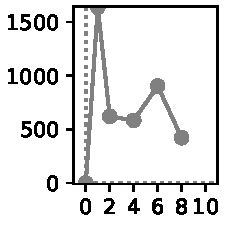
\includegraphics[width=0.3\textwidth]{figures/evaluateCross_BRIEF_SeparateEncoding.py_SimulateSynthetic_Parameterized_OtherNoiseLevels_Grid_VarySize_ZeroTrig_SeparateEncodings.py_180_0_2345_N40000_FOURIER_009_FOURIER_010-FOURIER_011-FOURIER_012-FOURIER_013.txt_RelativeLF.pdf}

\ 

Example 2 ($p=1$)

\sideimage{Original}{figures/CounterfactualModel_SeparateEncodings_VIZ.py_2345_FOURIER_109_FOURIER_110-FOURIER_111-FOURIER_112-FOURIER_113_1_0_10.0_180.pdf}



\sideimage{Fitted}{figures/RunSynthetic_FreePrior_L1Loss_OnSim_SeparateEncoding_VIZ.py_SimulateSynthetic_Parameterized_OtherNoiseLevels_Grid_VarySize_SeparateEncodings.py_180_1_2345_N40000_FOURIER_109_FOURIER_110-FOURIER_111-FOURIER_112-FOURIER_113.txt_1_0_10.0_180.pdf}

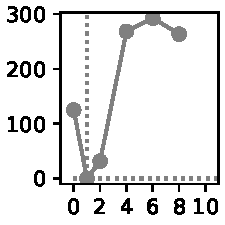
\includegraphics[width=0.3\textwidth]{figures/evaluateCrossValidationResults_Synthetic_Gardelle_NonF_SeparateEncoding.py_SimulateSynthetic_Parameterized_OtherNoiseLevels_Grid_VarySize_SeparateEncodings.py_180_1_2345_N40000_FOURIER_109_FOURIER_110-FOURIER_111-FOURIER_112-FOURIER_113.txt_RelativeLF.pdf}


\ 

Example 3 ($p=2$)

\sideimage{Original}{figures/CounterfactualModel_SeparateEncodings_VIZ.py_2345_FOURIER_209_FOURIER_210-FOURIER_211-FOURIER_212-FOURIER_213_2_0_10.0_180.pdf}
\sideimage{Fitted}{figures/RunSynthetic_FreePrior_CosineLoss_OnSim_SeparateEncoding_VIZ.py_SimulateSynthetic_Parameterized_OtherNoiseLevels_Grid_VarySize_SeparateEncodings.py_180_2_2345_N40000_FOURIER_209_FOURIER_210-FOURIER_211-FOURIER_212-FOURIER_213.txt_2_0_10.0_180.pdf}
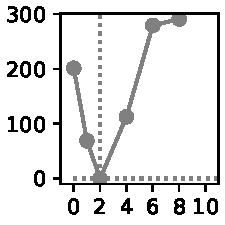
\includegraphics[width=0.3\textwidth]{figures/evaluateCrossValidationResults_Synthetic_Gardelle_NonF_SeparateEncoding.py_SimulateSynthetic_Parameterized_OtherNoiseLevels_Grid_VarySize_SeparateEncodings.py_180_2_2345_N40000_FOURIER_209_FOURIER_210-FOURIER_211-FOURIER_212-FOURIER_213.txt_RelativeLF.pdf}


  \end{minipage}%
  \hfill
  \begin{minipage}[b]{0.45\linewidth}
    \centering


Example 4 ($p=4$)

\sideimage{Original}{figures/CounterfactualModel_SeparateEncodings_VIZ.py_2345_FOURIER_409_FOURIER_410-FOURIER_411-FOURIER_412-FOURIER_413_4_0_10.0_180.pdf}
\sideimage{Fitted}{figures/RunSynthetic_FreePrior_CosineLoss_OnSim_SeparateEncoding_VIZ.py_SimulateSynthetic_Parameterized_OtherNoiseLevels_Grid_VarySize_SeparateEncodings.py_180_4_2345_N40000_FOURIER_409_FOURIER_410-FOURIER_411-FOURIER_412-FOURIER_413.txt_4_0_10.0_180.pdf}
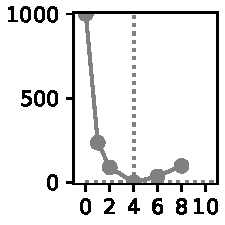
\includegraphics[width=0.3\textwidth]{figures/evaluateCrossValidationResults_Synthetic_Gardelle_NonF_SeparateEncoding.py_SimulateSynthetic_Parameterized_OtherNoiseLevels_Grid_VarySize_SeparateEncodings.py_180_4_2345_N40000_FOURIER_409_FOURIER_410-FOURIER_411-FOURIER_412-FOURIER_413.txt_RelativeLF.pdf}

\ 

Example 5 ($p=6$)

\sideimage{Original}{figures/CounterfactualModel_SeparateEncodings_VIZ.py_2345_FOURIER_609_FOURIER_610-FOURIER_611-FOURIER_612-FOURIER_613_6_0_10.0_180.pdf}
\sideimage{Fitted}{figures/RunSynthetic_FreePrior_CosineLoss_OnSim_SeparateEncoding_VIZ.py_SimulateSynthetic_Parameterized_OtherNoiseLevels_Grid_VarySize_SeparateEncodings.py_180_6_2345_N40000_FOURIER_609_FOURIER_610-FOURIER_611-FOURIER_612-FOURIER_613.txt_6_0_10.0_180.pdf}
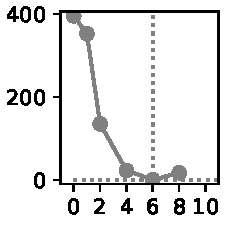
\includegraphics[width=0.3\textwidth]{figures/evaluateCrossValidationResults_Synthetic_Gardelle_NonF_SeparateEncoding.py_SimulateSynthetic_Parameterized_OtherNoiseLevels_Grid_VarySize_SeparateEncodings.py_180_6_2345_N40000_FOURIER_609_FOURIER_610-FOURIER_611-FOURIER_612-FOURIER_613.txt_RelativeLF.pdf}

\ 

Example 6 ($p=8$)






\sideimage{Original}{figures/CounterfactualModel_SeparateEncodings_VIZ.py_2345_FOURIER_809_FOURIER_810-FOURIER_811-FOURIER_812-FOURIER_813_8_0_10.0_180.pdf}
\sideimage{Fitted}{figures/RunSynthetic_FreePrior_CosineLoss_OnSim_SeparateEncoding_VIZ.py_SimulateSynthetic_Parameterized_OtherNoiseLevels_Grid_VarySize_SeparateEncodings.py_180_8_2345_N40000_FOURIER_809_FOURIER_810-FOURIER_811-FOURIER_812-FOURIER_813.txt_8_0_10.0_180.pdf}
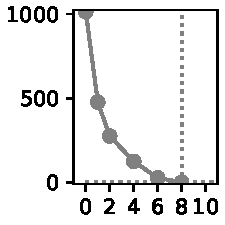
\includegraphics[width=0.3\textwidth]{figures/evaluateCrossValidationResults_Synthetic_Gardelle_NonF_SeparateEncoding.py_SimulateSynthetic_Parameterized_OtherNoiseLevels_Grid_VarySize_SeparateEncodings.py_180_8_2345_N40000_FOURIER_809_FOURIER_810-FOURIER_811-FOURIER_812-FOURIER_813.txt_RelativeLF.pdf}

\end{minipage}



\caption{Models may be identifiable even when the encoding varies between noise conditions. Here, the encoding resources are independently randomly generated in each noise condition, while the prior is shared across conditions. Even in this situation, the ground-truth loss function can be identified.}\label{fig:encoding-varies-fourier}
\end{figure}







\end{document}
